% Semiseparable transfer-matrix mask — TikZ source. Compiles to a tight standalone
% PDF (pdflatex figures/semiseparable-mask.tex), which `book-scaffold build-figures`
% converts to public/figures/semiseparable-mask.svg (PDF -> SVG via pdftocairo).
%
% The n=8, chunk-size c=4 transfer matrix T of a selective SSM: zero above the
% diagonal (causality), two dense c-by-c diagonal tiles (intra-chunk masked
% matmuls, shaded by the decay L_ij = prod a_s toward each tile's own diagonal),
% and the sub-diagonal c-by-c rectangle of rank at most d_s, every entry of
% which factors through the boundary state h_p at the chunk seam p=4. Tiling
% the diagonal densely and scanning boundary states IS the chunked algorithm;
% the footer states the duality factorization T = L o (CB^T)diag(Delta).
\documentclass[tikz,border=3pt]{standalone}
\usepackage{amsmath}
\usepackage{amssymb}
\usepackage{tikz}
\usetikzlibrary{positioning,arrows.meta,calc}
\begin{document}
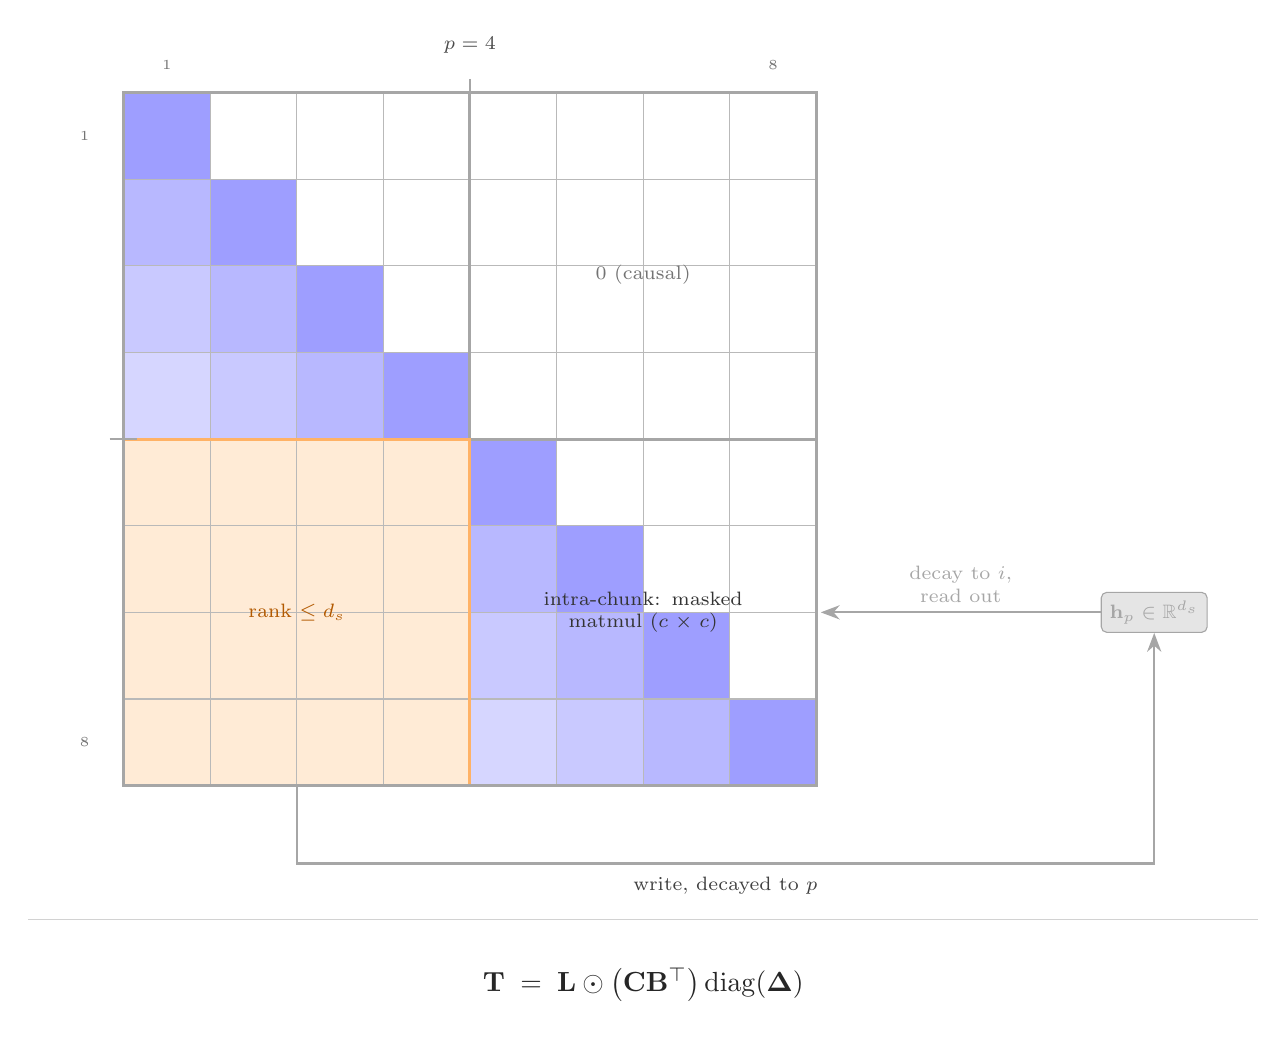
\begin{tikzpicture}[
    x=11mm, y=11mm,
    font=\small,
    op/.style={->, >={Stealth[length=2.4mm]}, gray!70, thick},
    state/.style={draw, gray!70, rounded corners=2pt, fill=black!10,
                  inner sep=3pt, font=\scriptsize, align=center},
    blbl/.style={font=\scriptsize, align=center, text=black!80},
  ]

  % ---------- cell grid: row i=1..8 top-down, col j=1..8 left-right;
  % cell (i,j) occupies x in [j-1,j], y in [1-i,-i] ----------
  \foreach \i in {1,...,8} {
    \foreach \j in {1,...,8} {
      \pgfmathtruncatemacro{\rankblk}{(\i>4 && \j<5) ? 1 : 0}
      \ifnum\j>\i
        \fill[white] (\j-1,1-\i) rectangle ++(1,-1);
      \else
        \ifnum\rankblk=1
          \fill[orange!16] (\j-1,1-\i) rectangle ++(1,-1);
        \else
          \pgfmathtruncatemacro{\shade}{38*pow(0.75,\i-\j)}
          \fill[blue!\shade] (\j-1,1-\i) rectangle ++(1,-1);
        \fi
      \fi
      \draw[gray!55] (\j-1,1-\i) rectangle ++(1,-1);
    }
  }

  % ---------- block frames ----------
  \draw[gray!70, line width=1.1pt] (0,0) rectangle (4,-4);    % block A (chunk 1)
  \draw[gray!70, line width=1.1pt] (4,-4) rectangle (8,-8);   % block B (chunk 2)
  \draw[orange!60, line width=1.1pt] (0,-4) rectangle (4,-8); % rank <= d_s block
  \draw[gray!70, line width=0.9pt] (0,0) rectangle (8,-8);    % outer frame

  % ---------- axis index labels (corners only) ----------
  \node[font=\tiny, text=black!55] at (-0.45,-0.5) {$1$};
  \node[font=\tiny, text=black!55] at (-0.45,-7.5) {$8$};
  \node[font=\tiny, text=black!55] at (0.5,0.32) {$1$};
  \node[font=\tiny, text=black!55] at (7.5,0.32) {$8$};

  % ---------- chunk-boundary tick at p = 4 ----------
  \draw[gray!70, thick] (4,0.16) -- (4,-0.16);
  \draw[gray!70, thick] (-0.16,-4) -- (0.16,-4);
  \node[font=\scriptsize, text=black!70] at (4,0.55) {$p=4$};

  % ---------- causal annotation ----------
  \node[font=\scriptsize, text=black!55, align=center] at (6,-2.1) {$0$ (causal)};

  % ---------- diagonal-block / rank-block labels ----------
  \node[blbl, text width=27mm] at (6,-6) {intra-chunk: masked\\matmul ($c\times c$)};
  \node[blbl, text=orange!70!black] at (2,-6) {rank $\le d_s$};

  % ---------- boundary-state node + write/read arrows ----------
  \node[state] (hp) at (11.9,-6) {$\mathbf h_p\in\mathbb R^{d_s}$};
  \draw[op] (hp.west) -- (8.05,-6)
    node[midway, above, font=\scriptsize, align=center] {decay to $i$,\\read out};
  \draw[op] (2,-8) -- (2,-8.9) -- (11.9,-8.9) -- (hp.south);
  \node[font=\scriptsize, text=black!75] at (6.95,-9.15) {write, decayed to $p$};

  % ---------- footer formula strip ----------
  \draw[gray!35] (-1.1,-9.55) -- (13.1,-9.55);
  \node[font=\normalsize, text=black!85] at (6,-10.3)
    {$\mathbf T \;=\; \mathbf L \odot \bigl(\mathbf C\mathbf B^{\top}\bigr)\operatorname{diag}(\boldsymbol\Delta)$};

\end{tikzpicture}
\end{document}
